%  LaTeX support: latex@mdpi.com 
%  For support, please attach all files needed for compiling as well as the log file, and specify your operating system, LaTeX version, and LaTeX editor.

%=================================================================
\documentclass[journal,article,submit,pdftex,moreauthors]{Definitions/mdpi} 

%--------------------
% Class Options:
%--------------------
%----------
% journal
%----------
% Choose between the following MDPI journals:
% acoustics, actuators, addictions, admsci, adolescents, aerobiology, aerospace, agriculture, agriengineering, agrochemicals, agronomy, ai, air, algorithms, allergies, alloys, analytica, analytics, anatomia, animals, antibiotics, antibodies, antioxidants, applbiosci, appliedchem, appliedmath, applmech, applmicrobiol, applnano, applsci, aquacj, architecture, arm, arthropoda, arts, asc, asi, astronomy, atmosphere, atoms, audiolres, automation, axioms, bacteria, batteries, bdcc, behavsci, beverages, biochem, bioengineering, biologics, biology, biomass, biomechanics, biomed, biomedicines, biomedinformatics, biomimetics, biomolecules, biophysica, biosensors, biotech, birds, bloods, blsf, brainsci, breath, buildings, businesses, cancers, carbon, cardiogenetics, catalysts, cells, ceramics, challenges, chemengineering, chemistry, chemosensors, chemproc, children, chips, cimb, civileng, cleantechnol, climate, clinpract, clockssleep, cmd, coasts, coatings, colloids, colorants, commodities, compounds, computation, computers, condensedmatter, conservation, constrmater, cosmetics, covid, crops, cryptography, crystals, csmf, ctn, curroncol, cyber, dairy, data, ddc, dentistry, dermato, dermatopathology, designs, devices, diabetology, diagnostics, dietetics, digital, disabilities, diseases, diversity, dna, drones, dynamics, earth, ebj, ecologies, econometrics, economies, education, ejihpe, electricity, electrochem, electronicmat, electronics, encyclopedia, endocrines, energies, eng, engproc, entomology, entropy, environments, environsciproc, epidemiologia, epigenomes, est, fermentation, fibers, fintech, fire, fishes, fluids, foods, forecasting, forensicsci, forests, foundations, fractalfract, fuels, future, futureinternet, futurepharmacol, futurephys, futuretransp, galaxies, games, gases, gastroent, gastrointestdisord, gels, genealogy, genes, geographies, geohazards, geomatics, geosciences, geotechnics, geriatrics, grasses, gucdd, hazardousmatters, healthcare, hearts, hemato, hematolrep, heritage, higheredu, highthroughput, histories, horticulturae, hospitals, humanities, humans, hydrobiology, hydrogen, hydrology, hygiene, idr, ijerph, ijfs, ijgi, ijms, ijns, ijpb, ijtm, ijtpp, ime, immuno, informatics, information, infrastructures, inorganics, insects, instruments, inventions, iot, j, jal, jcdd, jcm, jcp, jcs, jcto, jdb, jeta, jfb, jfmk, jimaging, jintelligence, jlpea, jmmp, jmp, jmse, jne, jnt, jof, joitmc, jor, journalmedia, jox, jpm, jrfm, jsan, jtaer, jvd, jzbg, kidneydial, kinasesphosphatases, knowledge, land, languages, laws, life, liquids, literature, livers, logics, logistics, lubricants, lymphatics, machines, macromol, magnetism, magnetochemistry, make, marinedrugs, materials, materproc, mathematics, mca, measurements, medicina, medicines, medsci, membranes, merits, metabolites, metals, meteorology, methane, metrology, micro, microarrays, microbiolres, micromachines, microorganisms, microplastics, minerals, mining, modelling, molbank, molecules, mps, msf, mti, muscles, nanoenergyadv, nanomanufacturing,\gdef\@continuouspages{yes}} nanomaterials, ncrna, ndt, network, neuroglia, neurolint, neurosci, nitrogen, notspecified, %%nri, nursrep, nutraceuticals, nutrients, obesities, oceans, ohbm, onco, %oncopathology, optics, oral, organics, organoids, osteology, oxygen, parasites, parasitologia, particles, pathogens, pathophysiology, pediatrrep, pharmaceuticals, pharmaceutics, pharmacoepidemiology,\gdef\@ISSN{2813-0618}\gdef\@continuous pharmacy, philosophies, photochem, photonics, phycology, physchem, physics, physiologia, plants, plasma, platforms, pollutants, polymers, polysaccharides, poultry, powders, preprints, proceedings, processes, prosthesis, proteomes, psf, psych, psychiatryint, psychoactives, publications, quantumrep, quaternary, qubs, radiation, reactions, receptors, recycling, regeneration, religions, remotesensing, reports, reprodmed, resources, rheumato, risks, robotics, ruminants, safety, sci, scipharm, sclerosis, seeds, sensors, separations, sexes, signals, sinusitis, skins, smartcities, sna, societies, socsci, software, soilsystems, solar, solids, spectroscj, sports, standards, stats, std, stresses, surfaces, surgeries, suschem, sustainability, symmetry, synbio, systems, targets, taxonomy, technologies, telecom, test, textiles, thalassrep, thermo, tomography, tourismhosp, toxics, toxins, transplantology, transportation, traumacare, traumas, tropicalmed, universe, urbansci, uro, vaccines, vehicles, venereology, vetsci, vibration, virtualworlds, viruses, vision, waste, water, wem, wevj, wind, women, world, youth, zoonoticdis 
% For posting an early version of this manuscript as a preprint, you may use "preprints" as the journal. Changing "submit" to "accept" before posting will remove line numbers.

%---------
% article
%---------
% The default type of manuscript is "article", but can be replaced by: 
% abstract, addendum, article, book, bookreview, briefreport, casereport, comment, commentary, communication, conferenceproceedings, correction, conferencereport, entry, expressionofconcern, extendedabstract, datadescriptor, editorial, essay, erratum, hypothesis, interestingimage, obituary, opinion, projectreport, reply, retraction, review, perspective, protocol, shortnote, studyprotocol, systematicreview, supfile, technicalnote, viewpoint, guidelines, registeredreport, tutorial
% supfile = supplementary materials

%----------
% submit
%----------
% The class option "submit" will be changed to "accept" by the Editorial Office when the paper is accepted. This will only make changes to the frontpage (e.g., the logo of the journal will get visible), the headings, and the copyright information. Also, line numbering will be removed. Journal info and pagination for accepted papers will also be assigned by the Editorial Office.

%------------------
% moreauthors
%------------------
% If there is only one author the class option oneauthor should be used. Otherwise use the class option moreauthors.

%---------
% pdftex
%---------
% The option pdftex is for use with pdfLaTeX. Remove "pdftex" for (1) compiling with LaTeX & dvi2pdf (if eps figures are used) or for (2) compiling with XeLaTeX.

%=================================================================
% MDPI internal commands - do not modify
\firstpage{1} 
\makeatletter 
\setcounter{page}{\@firstpage} 
\makeatother
\pubvolume{1}
\issuenum{1}
\articlenumber{0}
\pubyear{2023}
\copyrightyear{2023}
%\externaleditor{Academic Editor: Firstname Lastname}
\datereceived{ } 
\daterevised{ } % Comment out if no revised date
\dateaccepted{ } 
\datepublished{ } 
%\datecorrected{} % For corrected papers: "Corrected: XXX" date in the original paper.
%\dateretracted{} % For corrected papers: "Retracted: XXX" date in the original paper.
\hreflink{https://doi.org/} % If needed use \linebreak
%\doinum{}
%\pdfoutput=1 % Uncommented for upload to arXiv.org

%=================================================================
% Add packages and commands here. The following packages are loaded in our class file: fontenc, inputenc, calc, indentfirst, fancyhdr, graphicx, epstopdf, lastpage, ifthen, float, amsmath, amssymb, lineno, setspace, enumitem, mathpazo, booktabs, titlesec, etoolbox, tabto, xcolor, colortbl, soul, multirow, microtype, tikz, totcount, changepage, attrib, upgreek, array, tabularx, pbox, ragged2e, tocloft, marginnote, marginfix, enotez, amsthm, natbib, hyperref, cleveref, scrextend, url, geometry, newfloat, caption, draftwatermark, seqsplit
% cleveref: load \crefname definitions after \begin{document}
\usepackage{caption}
\usepackage{subcaption}
\usepackage{algorithm}
\usepackage{algpseudocode}
%=================================================================
% Please use the following mathematics environments: Theorem, Lemma, Corollary, Proposition, Characterization, Property, Problem, Example, ExamplesandDefinitions, Hypothesis, Remark, Definition, Notation, Assumption
%% For proofs, please use the proof environment (the amsthm package is loaded by the MDPI class).

%=================================================================
% Full title of the paper (Capitalized)
\Title{Title}

% MDPI internal command: Title for citation in the left column
\TitleCitation{Title}

% Author Orchid ID: enter ID or remove command
\newcommand{\orcidauthorA}{0000-0000-0000-000X} % Add \orcidA{} behind the author's name
%\newcommand{\orcidauthorB}{0000-0000-0000-000X} % Add \orcidB{} behind the author's name

% Authors, for the paper (add full first names)
\Author{Gianluca Massei $^{1,\dagger,\ddagger}$\orcidA{}, Giovanni Fioretti $^{2,\ddagger}$, Francesco A.N. Palmieri $^{2}$ $^{2,}$*,Francesco Verolla $^{2}$, Giovannio Di Gennaro$^{2}$ and Amedeo Buonanno $^{3}$}

%\longauthorlist{yes}

% MDPI internal command: Authors, for metadata in PDF
\AuthorNames{Gianluca Massei, Giovanni Fioretti , Francesco A.N. Palmieri, Giovanni Di Gennaro, Francesco Verolla and Amedeo Buonanno}

% MDPI internal command: Authors, for citation in the left column
\AuthorCitation{Massei, G.; Fioretti, G.; Verolla, F.; Palmieri, F., A.N., Di Gennaro, G. and Buonanno, A.}
% If this is a Chicago style journal: Lastname, Firstname, Firstname Lastname, and Firstname Lastname.

% Affiliations / Addresses (Add [1] after \address if there is only one affiliation.)
\address{%
$^{1}$ \quad CNIT\\
$^{2}$ \quad University of Campania Luigi Vanvitelli\\
$^{3}$ \quad ENEA\\
}

% Contact information of the corresponding author
\corres{Correspondence: gianluca.massei@cnit.it; Tel.: (optional; include country code; if there are multiple corresponding authors, add author initials) +xx-xxxx-xxx-xxxx (F.L.)}

% Current address and/or shared authorship
\firstnote{Current address: Affiliation 3.} 
\secondnote{These authors contributed equally to this work.}
% The commands \thirdnote{} till \eighthnote{} are available for further notes

%\simplesumm{} % Simple summary

%\conference{} % An extended version of a conference paper

% Abstract (Do not insert blank lines, i.e. \\) 
% A single paragraph of about 200 words maximum. For research articles, abstracts should give a pertinent overview of the work. We strongly encourage authors to use the following style of structured abstracts, but without headings: (1) Background: place the question addressed in a broad context and highlight the purpose of the study; (2) Methods: describe briefly the main methods or treatments applied; (3) Results: summarize the article's main findings; (4) Conclusions: indicate the main conclusions or interpretations. The abstract should be an objective representation of the article, it must not contain results which are not presented and substantiated in the main text and should not exaggerate the main conclusions.
\abstract{The proposed work aims to provide a path planning solution that use data about sea and weather conditions to find the optimal path the links 2 positions.}

% Keywords
\keyword{path planning; sea-state} 

% The fields PACS, MSC, and JEL may be left empty or commented out if not applicable
%\PACS{J0101}
%\MSC{}
%\JEL{}

%%%%%%%%%%%%%%%%%%%%%%%%%%%%%%%%%%%%%%%%%%
% Only for the journal Diversity
%\LSID{\url{http://}}

%%%%%%%%%%%%%%%%%%%%%%%%%%%%%%%%%%%%%%%%%%
% Only for the journal Applied Sciences
%\featuredapplication{Authors are encouraged to provide a concise description of the specific application or a potential application of the work. This section is not mandatory.}
%%%%%%%%%%%%%%%%%%%%%%%%%%%%%%%%%%%%%%%%%%

%%%%%%%%%%%%%%%%%%%%%%%%%%%%%%%%%%%%%%%%%%
% Only for the journal Data
%\dataset{DOI number or link to the deposited data set if the data set is published separately. If the data set shall be published as a supplement to this paper, this field will be filled by the journal editors. In this case, please submit the data set as a supplement.}
%\datasetlicense{License under which the data set is made available (CC0, CC-BY, CC-BY-SA, CC-BY-NC, etc.)}

%%%%%%%%%%%%%%%%%%%%%%%%%%%%%%%%%%%%%%%%%%
% Only for the journal Toxins
%\keycontribution{The breakthroughs or highlights of the manuscript. Authors can write one or two sentences to describe the most important part of the paper.}

%%%%%%%%%%%%%%%%%%%%%%%%%%%%%%%%%%%%%%%%%%
% Only for the journal Encyclopedia
%\encyclopediadef{For entry manuscripts only: please provide a brief overview of the entry title instead of an abstract.}

%%%%%%%%%%%%%%%%%%%%%%%%%%%%%%%%%%%%%%%%%%
% Only for the journal Advances in Respiratory Medicine
%\addhighlights{yes}
%\renewcommand{\addhighlights}{%

%\noindent This is an obligatory section in “Advances in Respiratory Medicine”, whose goal is to increase the discoverability and readability of the article via search engines and other scholars. Highlights should not be a copy of the abstract, but a simple text allowing the reader to quickly and simplified find out what the article is about and what can be cited from it. Each of these parts should be devoted up to 2~bullet points.\vspace{3pt}\\
%\textbf{What are the main findings?}
% \begin{itemize}[labelsep=2.5mm,topsep=-3pt]
% \item First bullet.
% \item Second bullet.
% \end{itemize}\vspace{3pt}
%\textbf{What is the implication of the main finding?}
% \begin{itemize}[labelsep=2.5mm,topsep=-3pt]
% \item First bullet.
% \item Second bullet.
% \end{itemize}
%}

%%%%%%%%%%%%%%%%%%%%%%%%%%%%%%%%%%%%%%%%%%
\begin{document}

%%%%%%%%%%%%%%%%%%%%%%%%%%%%%%%%%%%%%%%%%%
% The order of the section titles is different for some journals. Please refer to the "Instructions for Authors” on the journal homepage.

\section{Introduction}
In recent years, robotics has been optimizing the monitoring and exploration of maritime and coastal scenarios through the use of multiple and sophisticated autonomous systems. 
This category includes the Autonomous Underwater Vehicles (AUV), underwater robots capable of completing missions autonomously, and the Autonomous Surface Vehicles (ASV), vehicles that rotate on the surface of the water without a crew. The application fields are various: geological prospecting, oceanographic monitoring, military sector, etc. 
Maritime navigation is an essential aspect of the shipping industry. Path planning in a maritime scenario is the process of determining the optimal route a vessel can take from the point of departure to the destination. 

The goal of this paper is to propose a new path planning method that uses a probability map to influence the final path according to sea-weather conditions.
The algorithm has bees tested on a real scenario, where the path planning has been performed in a maritime environment in the "Gulf of Naples" (Italy) according to 
the "\textbf{Progetto ARES - Autonomous Robotics for the Extended Ship}".
% \footnote[1]{https://www.cnit.it/progetti/progetti-nazionali/progetto-ares-robotica-autonoma-per-nave-estesa/}".
Our contribution to the project is the development part of a DSS (Decision Support System) that helps the operator during a mission by providing a path planning solution 
that takes into account sea-weather conditions.
The focus will be on discussing the various challenges that arise in this area and the proposed solutions to overcome them. 
The method will be compared to some state-of-the-art techniques too.


\subsection{State-of-the-art}
\colorbox{yellow}{TODO}

\subsection{WiP}

The path planning problem involves dealing with uncertain issues that affect from the actions taken by an agent. One expressway to accessibly represent and solve those kind of proglem is by utilizing 
a fine model called a Markov Decision Process(MDP). 
An MDP is outlined by a tuple  $\{T, \mathcal{S}, \mathcal{A}, p, r\}$, where $T$ is the time horizon, $\mathcal{S}$ a set of all possible states,
 $\mathcal{A}$ a set of all possible actions, $p$ is the state transition function and $r$ is the reward function.

In our work, we consider a discrete environment of size $N\times M$ and the considered agent can move in eight directions ($a_t$): up, down, left, right, and the four diagonal directions.
Using a discrete representation of the environment, each cell of the grid, that rapresent the possible states of the agent, can be associated with a variable $r(s_t, a_t)$ (Reward).
 The value of $r(s_t, a_t)$ is 1 if the cell is occupied and 0 if the cell is completly free of obstacles or 
a value between 0 and 1 whereever there is an higher or lower preference to move in that cell. This reward function guides the agent towards the optimal solution. 
For instance, for each time step $t$, the agent can be in a cell $s_t\in \mathcal{S}$ and can perform an action $a_t \in \mathcal{A}$ to move to a new state $s_{t+1}$ and it recive a reward 
$r(s_t, a_t) \in \mathcal{R}$.
The MDP based on state-action model can be rapresentated as a Bayseas Graph as shown in Figure \ref{fig:MDP}.

\begin{figure}
	\centering
	\includegraphics[width=0.7\textwidth]{res/imgs/Mdp.png}
	\caption{MDP}
	\label{fig:MDP}
\end{figure}



Our own algorithm is called \textit{Leader Algorithm} and it is based on the \textit{Leader-Follower} paradigm. It's a discrete and deterministic version of the Leader Algorithm outlined 
in \cite{}.\\
 
We will speak  of \textit {leader cell}. 

A $3 \times 3$ kernel centered on the leader cell is used for the diffusion process. All actions have a priority of $1$. 
Furthermore, the outcome of a given action is certain. In any case, the current implementation does not prohibit being able to condition these two characteristics.

A cell is updated as follows:
\begin{equation*}\label{eq:weight_update_disc}
    \nu_i = \nu(\mathcal{L}_i) + \log p(s,a) + R(s)
\end{equation*}
where $\nu_i$ is the value  of the new cell $i$, $\nu(\mathcal{L}_i)$ is the value of the leader cell, $\log p(s,a)$ is the value associated to the state-action pair(in particular, greater weight is given to steps taken diagonally) and $R(s)$ is the reward associated with the state $s$. Notice how, unlike the continuous version, the transition takes place in log-space.


\subsection{Our contribution}
\colorbox{yellow}{TODO}


\section{Module}
The proposed module works on successive steps:
\begin{itemize}[labelsep=2.5mm,topsep=-3pt]
	\item \textbf{Input data}: the developed module takes as input several parameters that are used to perform the path planning. 
	\item \textbf{Path planning}: the path planning is performed by using the developed module. 
	\item \textbf{Output data}: the developed module provides as output the path planning solution.
\end{itemize}

\subsection{Input data}
The developed module takes as input several sets of data divided into:
\begin{itemize}
\item Data for the construction of the parameterized map: wave motion 
\item Mission data: mission objectives, \colorbox{green}{NG Worker} start and goal positions, drone release positions(Intermediate positions), 
	mission duration, etc.;
\end{itemize}

\subsubsection{Data for the construction of the parameterized map}

All the weather data are provided by the \colorbox{green}{PARTHENOPE\footnote[2]{http://193.205.230.6:8080/opendap/hyrax/}}. The data are provided in the form of a netCDF file,
which is a self-describing file format that allows the storage of multidimensional arrays of scientific data and they are used to store both the map and the reward function.
The data that the module uses are:
\begin{itemize}
\item Significant height of wind and swell waves(see figure \ref*{fig:waveHeight}).
\item Peak direction(see figure \ref*{fig:pDir}).
\item Costal map(see figure \ref*{fig:coast}).
\end{itemize}

The significant height of the waves information has been used to get the informations about the Sea State.The term Sea State describes the general condition of the surface of the open sea. 
This is comprised of two core measurements, the wave height which is dependent on the local surface wind strength and thus termed the ‘wind sea’ and the swell which i
s a slow and regular movement of the sea in rolling waves that do not break and are in the process of dissipating as they travel from their relatively distant origin.\\
The sea state is described by the following chart: \\

\newcolumntype{C}{>{\centering\arraybackslash}X}
\begin{tabularx}{\textwidth}{CCC}
\toprule
\textbf{Code}	& \textbf{Height [m]}	& \textbf{Description}\\
\midrule
0		& no wave			& Calm (Glassy)\\
1		& 0 - 0.10			& Calm (Rippled) \\
2		& 0.10 - 0.50			& Smooth (Wavelets) \\
3		& 0.50 - 1.25			& Slight \\
4		& 1.25 - 2.50			& Moderate \\
5		& 2.50 - 4.00			& Rough \\
6		& 4.00 - 6.00			& Very Rough\\
7		& 6.00 - 9.00			&  High\\
8		& 9.00 - 14.00			& Very High \\
9		& 14.00+			& Phenomenal \\

\bottomrule
\end{tabularx}

Those informations are transformed in a probabilistic fashion using values from 0 to 1, where 0 means sea state 0 and 1 sea state greater or equal to 4.\\
Sea state greater then 4 are considered as the same because the considered agent (NG Worker) is not able to operate in those conditions.\\

The coast map is a binary map where 1 represents the presence of a coast and 0 the absence of a coast. This map has been processed applying a Gaussian filter to the original map 
to create a smooth transition between the coast and the sea to create different zones to avoiding collisions of the results path with the coast as shown in figure \ref*{fig:coastBlur}.\\
\begin{figure}[h]
	\begin{subfigure}{0.5\textwidth}
		\centering
		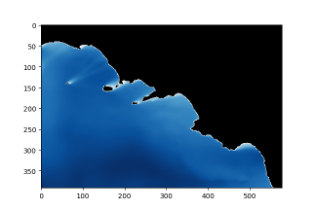
\includegraphics[width=\textwidth]{res/imgs/waveHeight.png}
		\caption{Wave height}
		\label{fig:waveHeight}
	\end{subfigure}
	\begin{subfigure}{0.5\textwidth}
		\centering
		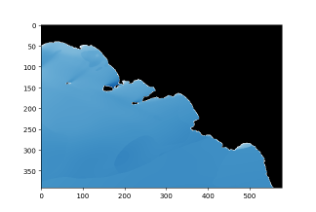
\includegraphics[width=\textwidth]{res/imgs/peakDir.png}
		\caption{Peak direction}
		\label{fig:pDir}
	\end{subfigure}
\end{figure}
\begin{figure}[h]
	\begin{subfigure}{0.5\textwidth}
		\centering
		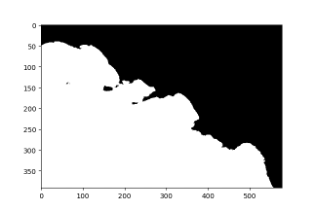
\includegraphics[width=\textwidth]{res/imgs/coast.png}
		\caption{Coast map}
		\label{fig:coast}
	\end{subfigure}
	\begin{subfigure}{0.5\textwidth}
		\centering
		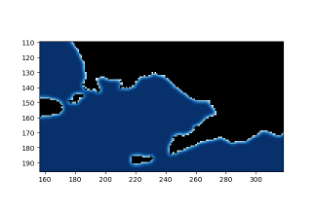
\includegraphics[width=\textwidth]{res/imgs/coastBlur.png}
		\caption{Coast map smoothed}
		\label{fig:coastBlur}
	\end{subfigure}
\end{figure}

All those parameters are combinated in a weighted sum and then normalizing the result in the range [0,1].\\
\begin{equation}
\label{eq:reward}
R(s_t) = \sum_{i=1}^n w_i \cdot f_i(s_t)
\end{equation}
where $s_t$ is the state at time $t$ and $f_i$ is the $i$-th information gained by the data and $w_i$ is the $i$-th weight.\\

\subsubsection{Mission data}
The mission data are the informations about the mission that the module has to solve. The mission data are:
\begin{itemize}
	\item The start position of the agent;
	\item The goal position of the agent;
	\item The optional release position of the drone;
\end{itemize}
Those informations can be provided by the user or by other DSS module through a MQTT message.\\
\colorbox{red}{le coordinate devono essere in lat e lon, da scrivere?}

\subsection{Algorithm}
To run the algorithm, as described previously the module needs the following information:
\begin{itemize}
	\item The start position of the agent;
	\item The goals position of the agent;
	\item The optional release position of the drone;
	\item The map of the area;
	\item The reward function;
	\item A set of actions that the agent can perform;
\end{itemize}

The actions that the agent can perform are the following: {move up, move down, move left, move right, move up-left, move up-right, move down-left, move down-right}.\\
The actions set is obtained through an euristic, thaking in consideration that the action of moving in diagonal is more expensive than the action of moving in a cardinal direction.\\
A time horizon $T$ is defined to limit the number of iteration of the algorithm (Stop criterion).\\
A phase of data collection and data processing is performed to obtain the reward function from the user input.\\
\colorbox{yellow}{Approfondire come si ottiene la reward function}\\
\colorbox{cyan}{Ricorda che la von mises é stata usata per modellare il fatto che l'agente deve preferire le azioni parallele alla direzione del fronte d'onda per non navigare contro corrente.}
Once all the data are collected, the computation starts. The cells of the map thet are goals are initialized with a reward of 1, the cells that are not goals are initialized with a reward of 0.
Using the update rule seen before, the reward of the cells are updated until the cell of the start position is reached (or the stop criterion is reached).\\

\begin{algorithm}
	\caption{Leader Algorithm}\label{alg:algorithm}
	\begin{algorithmic}
	\Require $T > 0$ \Comment{Time horizon}
	\State $A \gets Action Kernel  $ 
	\State $Map \gets Input data$
	\State $Reward \gets Reward update $
	\While{$ T \neq 0$}
		\State $Reward \gets Reward update $
		\State $T \gets T - 1$
	
	\EndWhile
	\end{algorithmic}
	\end{algorithm}

\colorbox{yellow}{TODO}

\subsection{Communication}
The communication between all the components of the DSS can comunicate through a MQTT broker.
MQTT or Message Queue Telemetry Transport is a featherlight and effective message protocol developed for the Internet of effects( IoT). 
It allows bias to change data in a publish- subscribe model, where data is published by a sender and entered by one or further subscribers. The protocol is grounded on a customer- garçon armature where guests can publish or subscribe to motifs on a garçon( also known as a broker). MQTT is ideal for IoT bias because it consumes minimum bandwidth and has low above, making it able for low- authority and resource- constrained bias. 
Its simplicity, scalability, and trustability have made it popular with inventors and has come a standard-issue protocol in the IoT assiduity.
An MQTT broker is a intermediary mecca that acts as a communication broker between MQTT guests. It's responsible for entering, storing, and ranking dispatches between guests. When an MQTT customer publishes a communication to a special content, the broker receives the communication and forwards it to all acceded guests that are interested in that content. also, when an MQTT customer subscribes to a content, the broker stores the subscription and forwards any dispatches published on that content to the acceded customer.

On the other phase, an MQTT customer is a device or operation that communicates with an MQTT broker. It can be either a publisher, subscriber, or both. When a customer publishes a communication to a special content, it sends the communication to the broker, which also on it to all acceded guests. When a customer subscribes to a content, it sends a subscription request to the broker, which stores the subscription and forwards any dispatches published on that content to the acceded customer.

In summary, the MQTT broker acts as an conciliator between MQTT guests, entering and ranking dispatches, while the MQTT guests are the bias or operations that give with the broker, publishing and assenting to dispatches. Together, the MQTT broker and guests form a publish- subscribe network, allowing effective and dependable message in IoT surroundings.


\colorbox{yellow}{TODO}

\section{Results}
\colorbox{yellow}{TODO}

\section{Conclusions}
\colorbox{yellow}{TODO}


%%%%%%%%%%%%%%%%%%%%%%%%%%%%%%%%%%%%%%%%%%
\section{Results}

This section may be divided by subheadings. It should provide a concise and precise description of the experimental results, their interpretation as well as the experimental conclusions that can be drawn.
\subsection{Subsection}
\subsubsection{Subsubsection}

Bulleted lists look like this:
\begin{itemize}
\item	First bullet;
\item	Second bullet;
\item	Third bullet.
\end{itemize}

Numbered lists can be added as follows:
\begin{enumerate}
\item	First item; 
\item	Second item;
\item	Third item.
\end{enumerate}

The text continues here. 

\subsection{Figures, Tables and Schemes}

All figures and tables should be cited in the main text as Figure~\ref{fig1}, Table~\ref{tab1}, etc.

\begin{figure}[H]

\includegraphics[width=10.5 cm]{Definitions/logo-mdpi}
\caption{This is a figure. Schemes follow the same formatting. If there are multiple panels, they should be listed as: (\textbf{a}) Description of what is contained in the first panel. (\textbf{b}) Description of what is contained in the second panel. Figures should be placed in the main text near to the first time they are cited. A caption on a single line should be centered.\label{fig1}}
\end{figure}   
\unskip

\begin{table}[H] 
\caption{This is a table caption. Tables should be placed in the main text near to the first time they are~cited.\label{tab1}}
\newcolumntype{C}{>{\centering\arraybackslash}X}
\begin{tabularx}{\textwidth}{CCC}
\toprule
\textbf{Title 1}	& \textbf{Title 2}	& \textbf{Title 3}\\
\midrule
Entry 1		& Data			& Data\\
Entry 2		& Data			& Data \textsuperscript{1}\\
\bottomrule
\end{tabularx}
\noindent{\footnotesize{\textsuperscript{1} Tables may have a footer.}}
\end{table}

The text continues here (Figure~\ref{fig2} and Table~\ref{tab2}).

% Example of a figure that spans the whole page width. The same concept works for tables, too.
\begin{figure}[H]
\begin{adjustwidth}{-\extralength}{0cm}
\centering

\includegraphics[width=15.5cm]{Definitions/logo-mdpi}
\end{adjustwidth}
\caption{This is a wide figure.\label{fig2}}
\end{figure}  

\begin{table}[H]
\caption{This is a wide table.\label{tab2}}
	\begin{adjustwidth}{-\extralength}{0cm}
		\newcolumntype{C}{>{\centering\arraybackslash}X}
		\begin{tabularx}{\fulllength}{CCCC}
			\toprule
			\textbf{Title 1}	& \textbf{Title 2}	& \textbf{Title 3}     & \textbf{Title 4}\\
			\midrule
\multirow[m]{3}{*}{Entry 1 *}	& Data			& Data			& Data\\
			  	                   & Data			& Data			& Data\\
			             	      & Data			& Data			& Data\\
                   \midrule
\multirow[m]{3}{*}{Entry 2}    & Data			& Data			& Data\\
			  	                  & Data			& Data			& Data\\
			             	     & Data			& Data			& Data\\
                   \midrule
\multirow[m]{3}{*}{Entry 3}    & Data			& Data			& Data\\
			  	                 & Data			& Data			& Data\\
			             	    & Data			& Data			& Data\\
                  \midrule
\multirow[m]{3}{*}{Entry 4}   & Data			& Data			& Data\\
			  	                 & Data			& Data			& Data\\
			             	    & Data			& Data			& Data\\
			\bottomrule
		\end{tabularx}
	\end{adjustwidth}
	\noindent{\footnotesize{* Tables may have a footer.}}
\end{table}

%\begin{listing}[H]
%\caption{Title of the listing}
%\rule{\columnwidth}{1pt}
%\raggedright Text of the listing. In font size footnotesize, small, or normalsize. Preferred format: left aligned and single spaced. Preferred border format: top border line and bottom border line.
%\rule{\columnwidth}{1pt}
%\end{listing}

Text.

Text.

\subsection{Formatting of Mathematical Components}

This is the example 1 of equation:
\begin{linenomath}
\begin{equation}
a = 1,
\end{equation}
\end{linenomath}
the text following an equation need not be a new paragraph. Please punctuate equations as regular text.
%% If the documentclass option "submit" is chosen, please insert a blank line before and after any math environment (equation and eqnarray environments). This ensures correct linenumbering. The blank line should be removed when the documentclass option is changed to "accept" because the text following an equation should not be a new paragraph.

This is the example 2 of equation:
\begin{adjustwidth}{-\extralength}{0cm}
\begin{equation}
a = b + c + d + e + f + g + h + i + j + k + l + m + n + o + p + q + r + s + t + u + v + w + x + y + z
\end{equation}
\end{adjustwidth}

% Example of a page in landscape format (with table and table footnote).
%\startlandscape
%\begin{table}[H] %% Table in wide page
%\caption{This is a very wide table.\label{tab3}}
%	\begin{tabularx}{\textwidth}{CCCC}
%		\toprule
%		\textbf{Title 1}	& \textbf{Title 2}	& \textbf{Title 3}	& \textbf{Title 4}\\
%		\midrule
%		Entry 1		& Data			& Data			& This cell has some longer content that runs over two lines.\\
%		Entry 2		& Data			& Data			& Data\textsuperscript{1}\\
%		\bottomrule
%	\end{tabularx}
%	\begin{adjustwidth}{+\extralength}{0cm}
%		\noindent\footnotesize{\textsuperscript{1} This is a table footnote.}
%	\end{adjustwidth}
%\end{table}
%\finishlandscape






%%%%%%%%%%%%%%%%%%%%%%%%%%%%%%%%%%%%%%%%%%
\section{Discussion}

Authors should discuss the results and how they can be interpreted from the perspective of previous studies and of the working hypotheses. The findings and their implications should be discussed in the broadest context possible. Future research directions may also be highlighted.

%%%%%%%%%%%%%%%%%%%%%%%%%%%%%%%%%%%%%%%%%%
\section{Conclusions}

This section is not mandatory, but can be added to the manuscript if the discussion is unusually long or complex.

%%%%%%%%%%%%%%%%%%%%%%%%%%%%%%%%%%%%%%%%%%
\section{Patents}

This section is not mandatory, but may be added if there are patents resulting from the work reported in this manuscript.

%%%%%%%%%%%%%%%%%%%%%%%%%%%%%%%%%%%%%%%%%%
\vspace{6pt} 

%%%%%%%%%%%%%%%%%%%%%%%%%%%%%%%%%%%%%%%%%%
%% optional
%\supplementary{The following supporting information can be downloaded at:  \linksupplementary{s1}, Figure S1: title; Table S1: title; Video S1: title.}

% Only for the journal Methods and Protocols:
% If you wish to submit a video article, please do so with any other supplementary material.
% \supplementary{The following supporting information can be downloaded at: \linksupplementary{s1}, Figure S1: title; Table S1: title; Video S1: title. A supporting video article is available at doi: link.}

%%%%%%%%%%%%%%%%%%%%%%%%%%%%%%%%%%%%%%%%%%
\authorcontributions{For research articles with several authors, a short paragraph specifying their individual contributions must be provided. The following statements should be used ``Conceptualization, X.X. and Y.Y.; methodology, X.X.; software, X.X.; validation, X.X., Y.Y. and Z.Z.; formal analysis, X.X.; investigation, X.X.; resources, X.X.; data curation, X.X.; writing---original draft preparation, X.X.; writing---review and editing, X.X.; visualization, X.X.; supervision, X.X.; project administration, X.X.; funding acquisition, Y.Y. All authors have read and agreed to the published version of the manuscript.'', please turn to the  \href{http://img.mdpi.org/data/contributor-role-instruction.pdf}{CRediT taxonomy} for the term explanation. Authorship must be limited to those who have contributed substantially to the work~reported.}

\funding{Please add: ``This research received no external funding'' or ``This research was funded by NAME OF FUNDER grant number XXX.'' and  and ``The APC was funded by XXX''. Check carefully that the details given are accurate and use the standard spelling of funding agency names at \url{https://search.crossref.org/funding}, any errors may affect your future funding.}

\institutionalreview{In this section, you should add the Institutional Review Board Statement and approval number, if relevant to your study. You might choose to exclude this statement if the study did not require ethical approval. Please note that the Editorial Office might ask you for further information. Please add “The study was conducted in accordance with the Declaration of Helsinki, and approved by the Institutional Review Board (or Ethics Committee) of NAME OF INSTITUTE (protocol code XXX and date of approval).” for studies involving humans. OR “The animal study protocol was approved by the Institutional Review Board (or Ethics Committee) of NAME OF INSTITUTE (protocol code XXX and date of approval).” for studies involving animals. OR “Ethical review and approval were waived for this study due to REASON (please provide a detailed justification).” OR “Not applicable” for studies not involving humans or animals.}

\informedconsent{Any research article describing a study involving humans should contain this statement. Please add ``Informed consent was obtained from all subjects involved in the study.'' OR ``Patient consent was waived due to REASON (please provide a detailed justification).'' OR ``Not applicable'' for studies not involving humans. You might also choose to exclude this statement if the study did not involve humans.

Written informed consent for publication must be obtained from participating patients who can be identified (including by the patients themselves). Please state ``Written informed consent has been obtained from the patient(s) to publish this paper'' if applicable.}

\dataavailability{We encourage all authors of articles published in MDPI journals to share their research data. In this section, please provide details regarding where data supporting reported results can be found, including links to publicly archived datasets analyzed or generated during the study. Where no new data were created, or where data is unavailable due to privacy or ethical re-strictions, a statement is still required. Suggested Data Availability Statements are available in section “MDPI Research Data Policies” at \url{https://www.mdpi.com/ethics}.} 

\acknowledgments{In this section you can acknowledge any support given which is not covered by the author contribution or funding sections. This may include administrative and technical support, or donations in kind (e.g., materials used for experiments).}

\conflictsofinterest{Declare conflicts of interest or state ``The authors declare no conflict of interest.'' Authors must identify and declare any personal circumstances or interest that may be perceived as inappropriately influencing the representation or interpretation of reported research results. Any role of the funders in the design of the study; in the collection, analyses or interpretation of data; in the writing of the manuscript; or in the decision to publish the results must be declared in this section. If there is no role, please state ``The funders had no role in the design of the study; in the collection, analyses, or interpretation of data; in the writing of the manuscript; or in the decision to publish the~results''.} 

%%%%%%%%%%%%%%%%%%%%%%%%%%%%%%%%%%%%%%%%%%
%% Optional
\sampleavailability{Samples of the compounds ... are available from the authors.}

%% Only for journal Encyclopedia
%\entrylink{The Link to this entry published on the encyclopedia platform.}

\abbreviations{Abbreviations}{
The following abbreviations are used in this manuscript:\\

\noindent 
\begin{tabular}{@{}ll}
MDPI & Multidisciplinary Digital Publishing Institute\\
DOAJ & Directory of open access journals\\
TLA & Three letter acronym\\
LD & Linear dichroism
\end{tabular}
}




\section[\appendixname~\thesection]{}
All appendix sections must be cited in the main text. In the appendices, Figures, Tables, etc. should be labeled, starting with ``A''---e.g., Figure A1, Figure A2, etc.

%%%%%%%%%%%%%%%%%%%%%%%%%%%%%%%%%%%%%%%%%%
\begin{adjustwidth}{-\extralength}{0cm}
%\printendnotes[custom] % Un-comment to print a list of endnotes

\reftitle{References}

% Please provide either the correct journal abbreviation (e.g. according to the “List of Title Word Abbreviations” http://www.issn.org/services/online-services/access-to-the-ltwa/) or the full name of the journal.
% Citations and References in Supplementary files are permitted provided that they also appear in the reference list here. 

%=====================================
% References, variant A: external bibliography
%=====================================
%\bibliography{your_external_BibTeX_file}

%=====================================
% References, variant B: internal bibliography
%=====================================
\begin{thebibliography}{999}
% Reference 1
\bibitem[Author1(year)]{ref-journal}
Author~1, T. The title of the cited article. {\em Journal Abbreviation} {\bf 2008}, {\em 10}, 142--149.
% Reference 2
\bibitem[Author2(year)]{ref-book1}
Author~2, L. The title of the cited contribution. In {\em The Book Title}; Editor 1, F., Editor 2, A., Eds.; Publishing House: City, Country, 2007; pp. 32--58.
% Reference 3
\bibitem[Author3(year)]{ref-book2}
Author 1, A.; Author 2, B. \textit{Book Title}, 3rd ed.; Publisher: Publisher Location, Country, 2008; pp. 154--196.
% Reference 4
\bibitem[Author4(year)]{ref-unpublish}
Author 1, A.B.; Author 2, C. Title of Unpublished Work. \textit{Abbreviated Journal Name} year, \textit{phrase indicating stage of publication (submitted; accepted; in press)}.
% Reference 5
\bibitem[Author5(year)]{ref-communication}
Author 1, A.B. (University, City, State, Country); Author 2, C. (Institute, City, State, Country). Personal communication, 2012.
% Reference 6
\bibitem[Author6(year)]{ref-proceeding}
Author 1, A.B.; Author 2, C.D.; Author 3, E.F. Title of presentation. In Proceedings of the Name of the Conference, Location of Conference, Country, Date of Conference (Day Month Year); Abstract Number (optional), Pagination (optional).
% Reference 7
\bibitem[Author7(year)]{ref-thesis}
Author 1, A.B. Title of Thesis. Level of Thesis, Degree-Granting University, Location of University, Date of Completion.
% Reference 8
\bibitem[Author8(year)]{ref-url}
Title of Site. Available online: URL (accessed on Day Month Year).
\end{thebibliography}

% If authors have biography, please use the format below
%\section*{Short Biography of Authors}
%\bio
%{\raisebox{-0.35cm}{\includegraphics[width=3.5cm,height=5.3cm,clip,keepaspectratio]{Definitions/author1.pdf}}}
%{\textbf{Firstname Lastname} Biography of first author}
%
%\bio
%{\raisebox{-0.35cm}{\includegraphics[width=3.5cm,height=5.3cm,clip,keepaspectratio]{Definitions/author2.jpg}}}
%{\textbf{Firstname Lastname} Biography of second author}

% For the MDPI journals use author-date citation, please follow the formatting guidelines on http://www.mdpi.com/authors/references
% To cite two works by the same author: \citeauthor{ref-journal-1a} (\citeyear{ref-journal-1a}, \citeyear{ref-journal-1b}). This produces: Whittaker (1967, 1975)
% To cite two works by the same author with specific pages: \citeauthor{ref-journal-3a} (\citeyear{ref-journal-3a}, p. 328; \citeyear{ref-journal-3b}, p.475). This produces: Wong (1999, p. 328; 2000, p. 475)

%%%%%%%%%%%%%%%%%%%%%%%%%%%%%%%%%%%%%%%%%%
%% for journal Sci
%\reviewreports{\\
%Reviewer 1 comments and authors’ response\\
%Reviewer 2 comments and authors’ response\\
%Reviewer 3 comments and authors’ response
%}
%%%%%%%%%%%%%%%%%%%%%%%%%%%%%%%%%%%%%%%%%%
\PublishersNote{}
\end{adjustwidth}
\end{document}
